\documentclass[aspectratio=169,11pt]{beamer}
\usetheme{default}\usecolortheme{seagull}\setbeamertemplate{navigation symbols}{}\setbeamertemplate{footline}{\hfill\scriptsize\insertframenumber/\inserttotalframenumber\hspace{2mm}\vspace{1mm}}
\usepackage[T1]{fontenc}\usepackage[utf8]{inputenc}\usepackage{lmodern}\usepackage{url}\usepackage{graphicx}
\setbeamerfont{frametitle}{size=\large,series=\bfseries}\setbeamercolor{frametitle}{fg=black}\setbeamertemplate{frametitle}{\vspace{2mm}\insertframetitle\par\vspace{1mm}\hrule}
\setbeamertemplate{itemize items}[circle]
\title{Le stationnement hors rue sur la rue de Terrebonne}\subtitle{Ce que montrent les plans d'assurance-incendie de 1954--1955, l'imagerie aérienne d'aujourd'hui et le LiDAR de la Ville, bâtiment par bâtiment}\author{Terrebonne-open-sources (un résident de Côte-des-Neiges--Notre-Dame-de-Grâce) \quad 2026-10-25}\date{}
\begin{document}
\begin{frame}\titlepage\vfill{\tiny Source\,: Underwriters' Survey Bureau, Insurance plan of the city of Montreal, vol.~7, 1954--1955 (BAnQ, notice 0000174390). Lecture\,: l'auteur, une ligne par bâtiment. Imagerie\,: Gouvernement du Québec (Imagerie\_GQ, consultée le 25 oct. 2026). LiDAR\,: Ville de Montréal 2015, CC-BY 4.0.}\end{frame}
\begin{frame}{60\,\% des bâtiments de la rue de Terrebonne ont été construits avec un garage}\begin{columns}[T]\column{0.6\textwidth}\begin{itemize}\item 126 bâtiments résidentiels adressés sur Terrebonne, de l'extrémité ouest de la piste à Girouard, sur les seize feuillets disponibles de 1954--1955
\item 75 construits avec un garage (côté nord 57 sur 90, côté sud 18 sur 36)
\item Par logements (rôle de la Ville)\,: 192 sur 324, 59\,\%
\item Les plans marquent les garages, pas les entrées\,: une borne inférieure pour «\,garage ou entrée d'origine\,»\end{itemize}\column{0.38\textwidth}\centering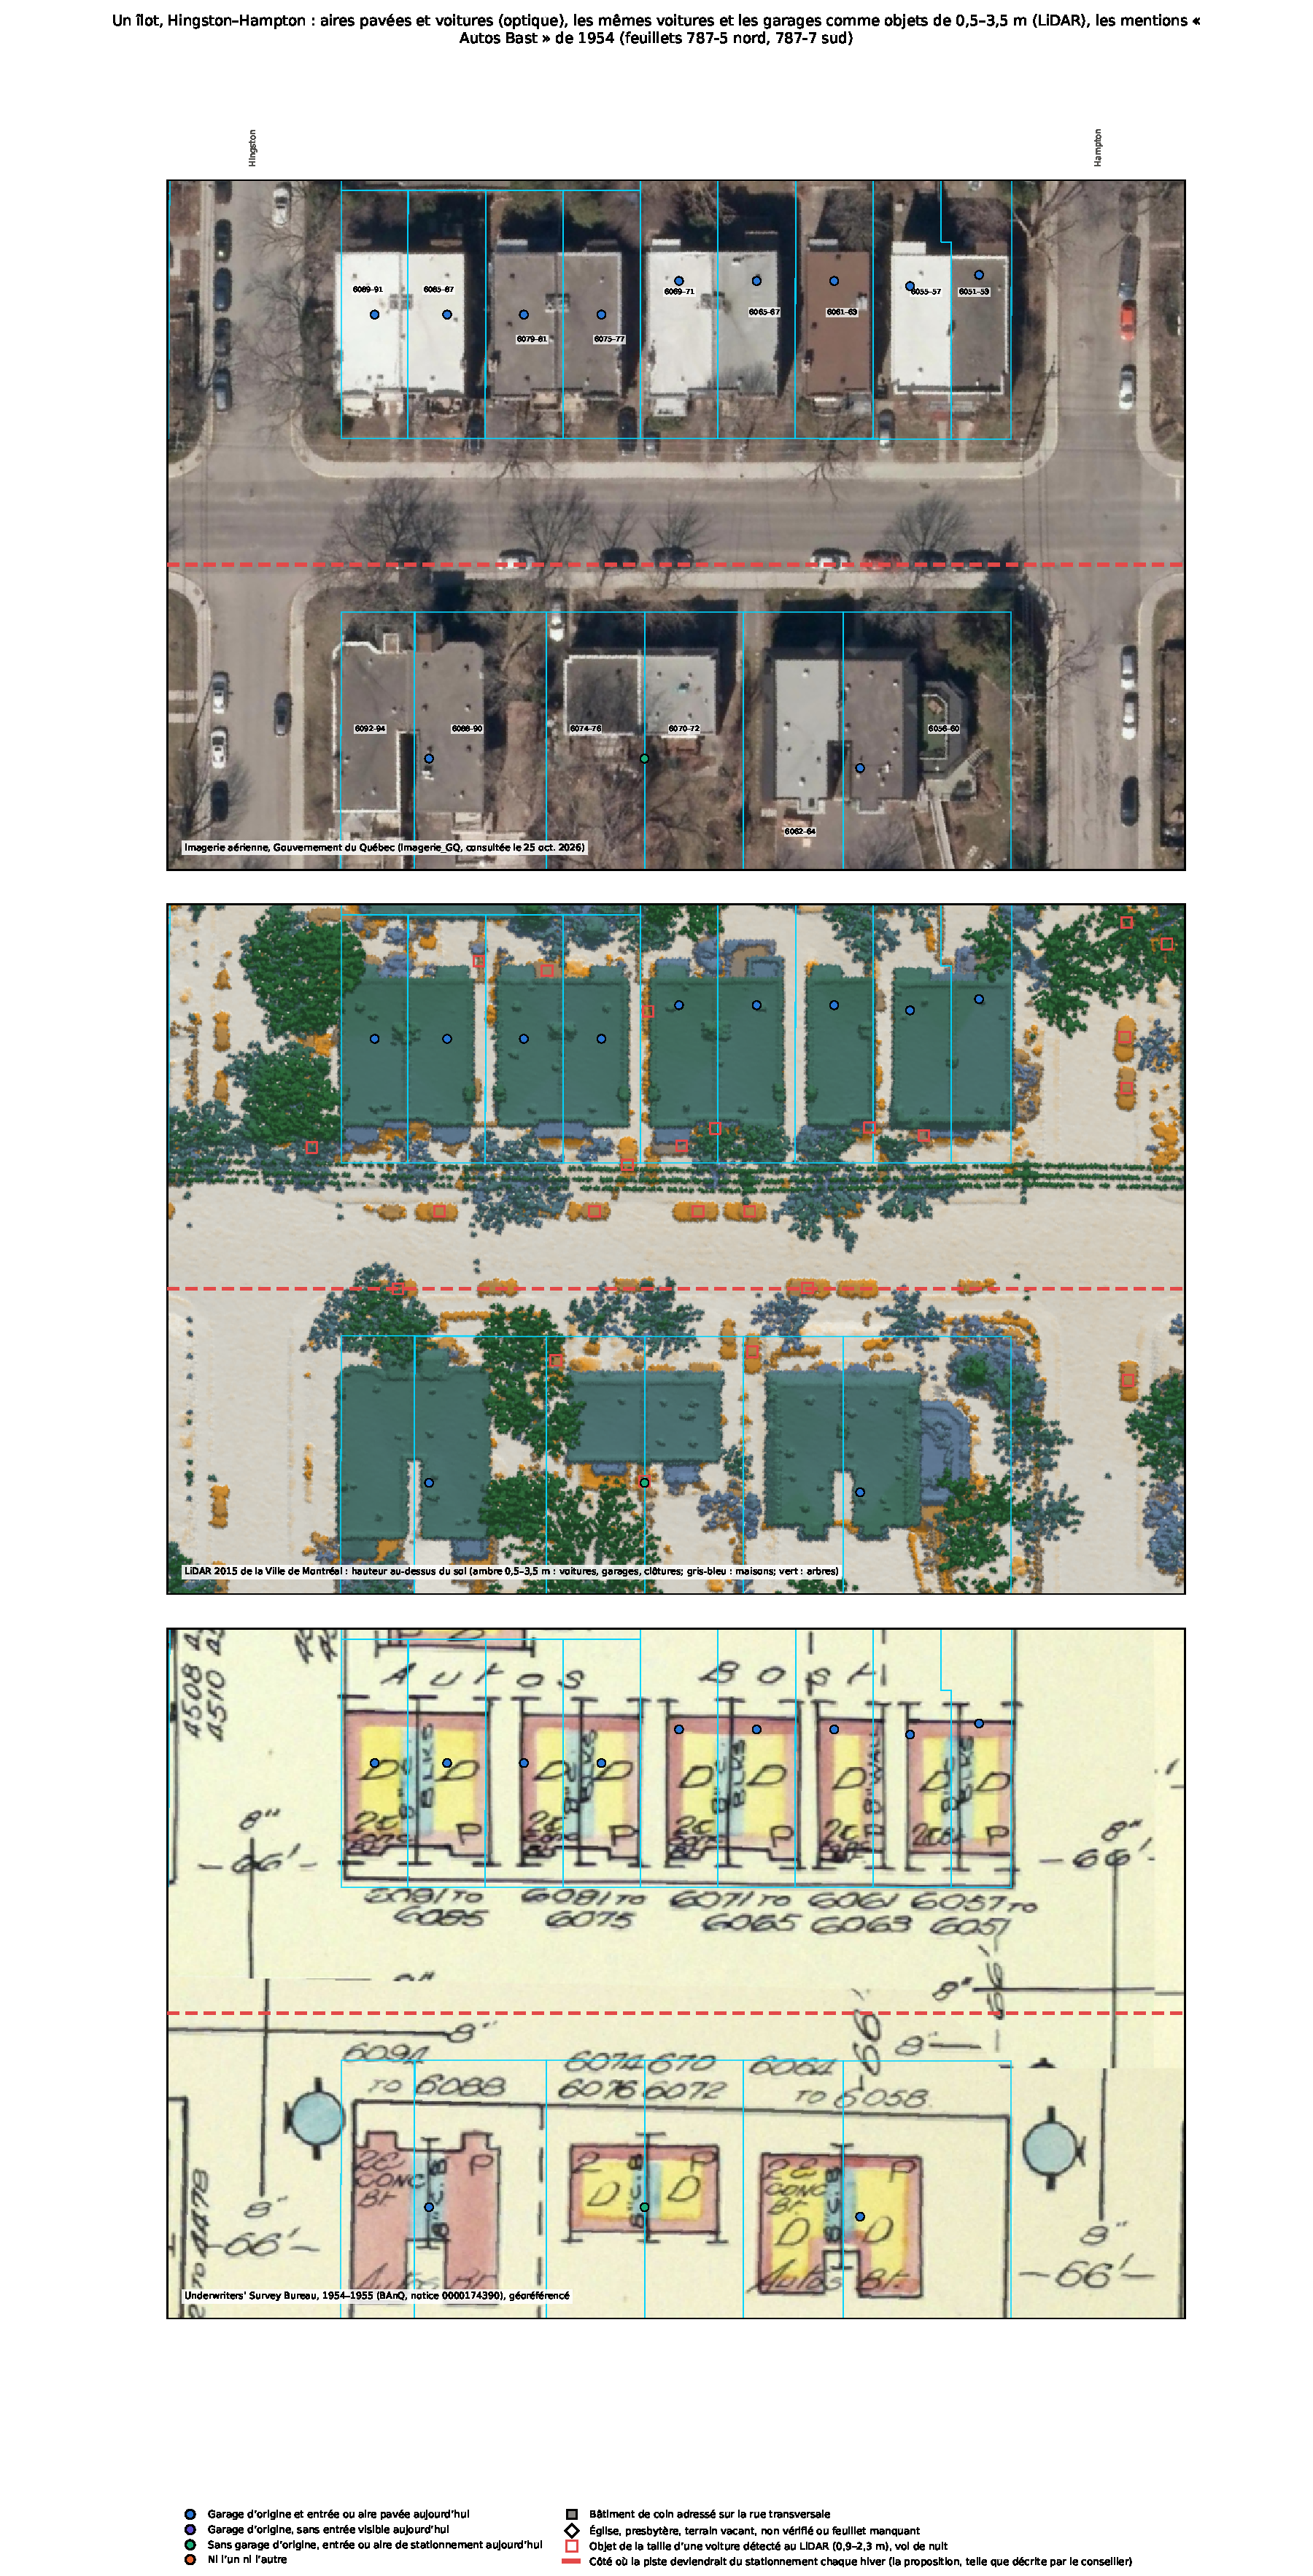
\includegraphics[height=0.68\textheight]{figures/method_detail_hingston_hampton_fr.pdf}\end{columns}\vfill{\tiny Source\,: Underwriters' Survey Bureau, Insurance plan of the city of Montreal, vol.~7, 1954--1955 (BAnQ, notice 0000174390). Lecture\,: l'auteur, une ligne par bâtiment.}\end{frame}
\begin{frame}{Aujourd'hui, 72\,\% ont un garage d'origine ou une entrée visible}\begin{itemize}\item 123 bâtiments vérifiés sur l'imagerie aérienne du Gouvernement du Québec (sans feuilles, 8\,cm par pixel, après juin 2024)
\item 79 montrent une entrée, une aire pavée ou une aire de stationnement (64\,\%)
\item Garage d'origine \emph{ou} entrée aujourd'hui\,: 89 sur 123 (72\,\%); par logements 73\,\%
\item Des garages de 1954, 64 gardent une aire visible, 10 non; 15 maisons sans garage en 1954 ont une entrée aujourd'hui
\item Ce qu'un garage contient ne se voit pas du ciel\end{itemize}\vfill{\tiny Imagerie\,: Gouvernement du Québec (Imagerie\_GQ, consultée le 25 oct. 2026). LiDAR\,: Ville de Montréal 2015, CC-BY 4.0. Fond\,: données ouvertes de la Ville de Montréal, CC-BY 4.0 (géobase, rôle d'évaluation). Lecture\,: l'auteur.}\end{frame}
\begin{frame}{Où sont les garages et les entrées, le long de toute la rue}\begin{center}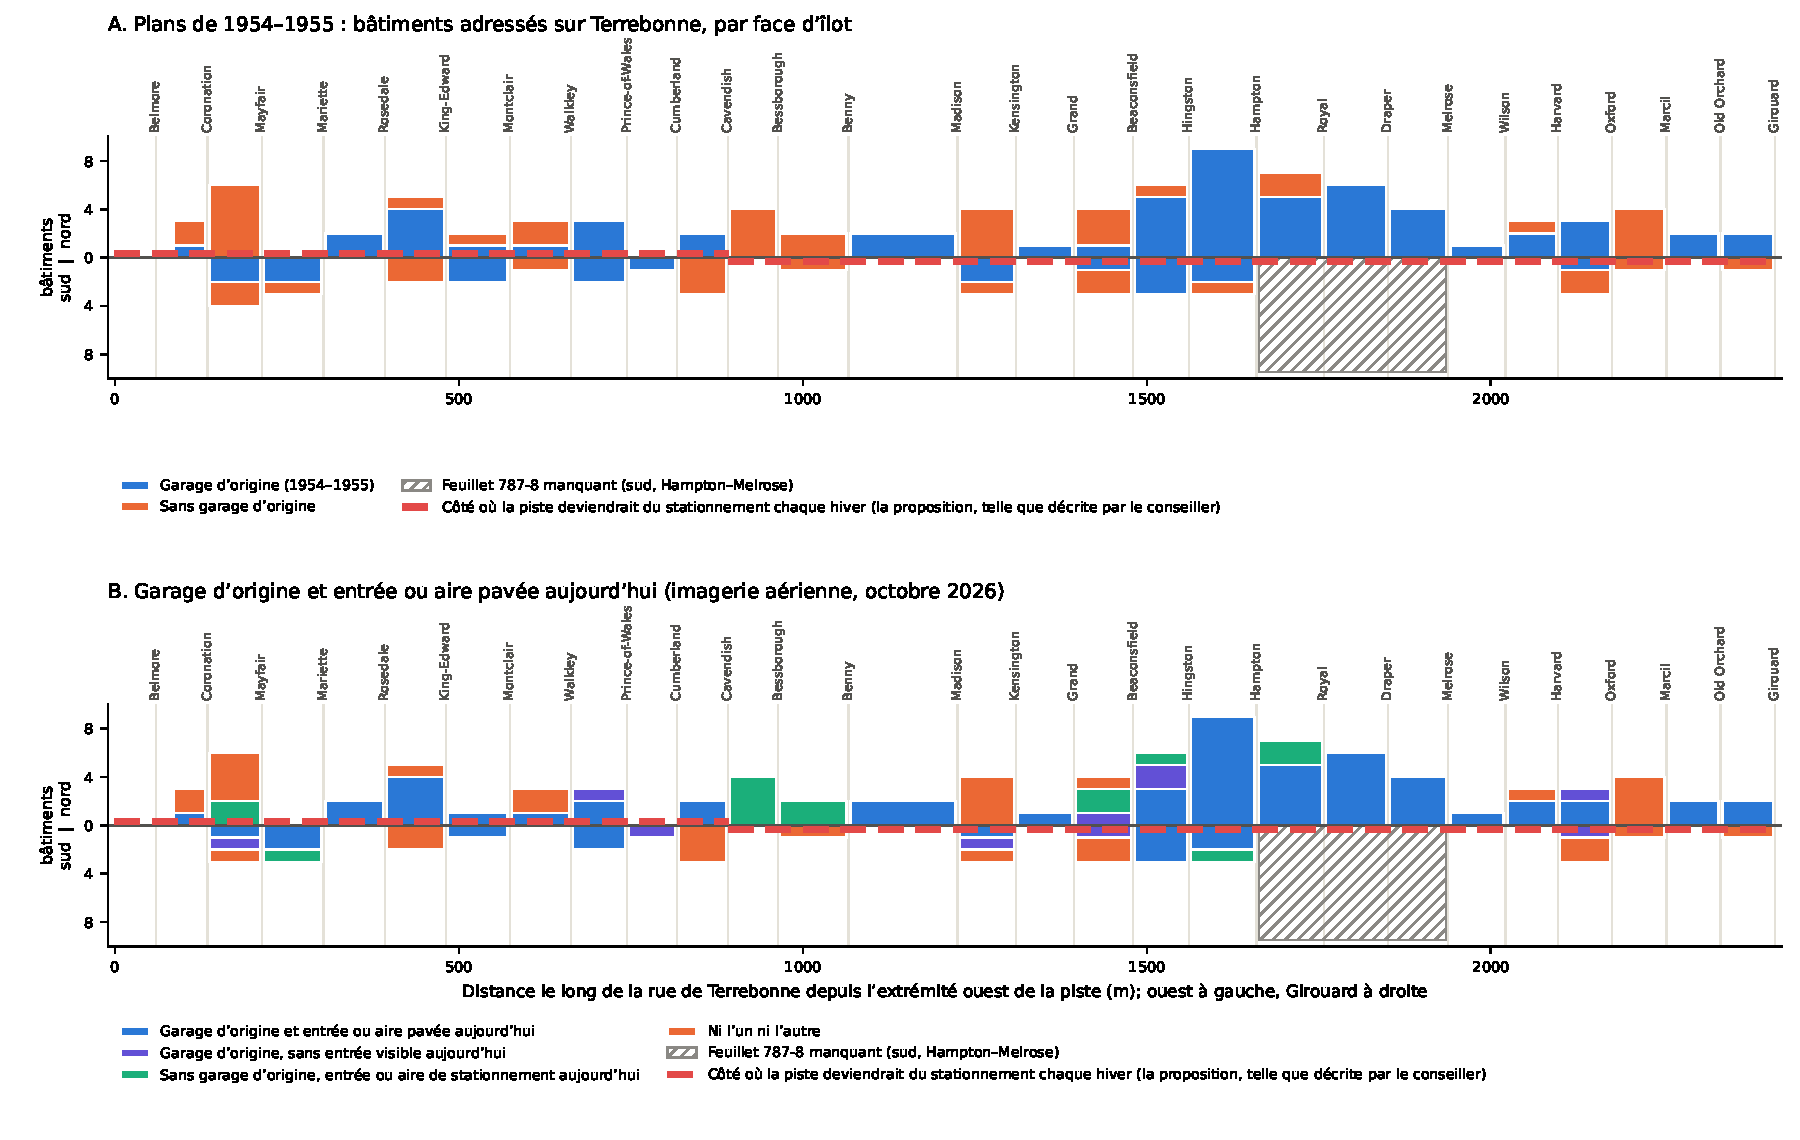
\includegraphics[height=0.72\textheight]{figures/terrebonne_garages_distribution_fr.pdf}\end{center}\vfill{\scriptsize Tirets rouges\,: le côté où la piste deviendrait du stationnement chaque hiver selon la proposition, telle que décrite par le conseiller.}\\{\tiny Source\,: Underwriters' Survey Bureau, Insurance plan of the city of Montreal, vol.~7, 1954--1955 (BAnQ, notice 0000174390). Lecture\,: l'auteur, une ligne par bâtiment. Imagerie\,: Gouvernement du Québec (Imagerie\_GQ, consultée le 25 oct. 2026). LiDAR\,: Ville de Montréal 2015, CC-BY 4.0.}\end{frame}
\begin{frame}{Sur le cadastre d'aujourd'hui\,: garage d'origine et entrée aujourd'hui}
\begin{center}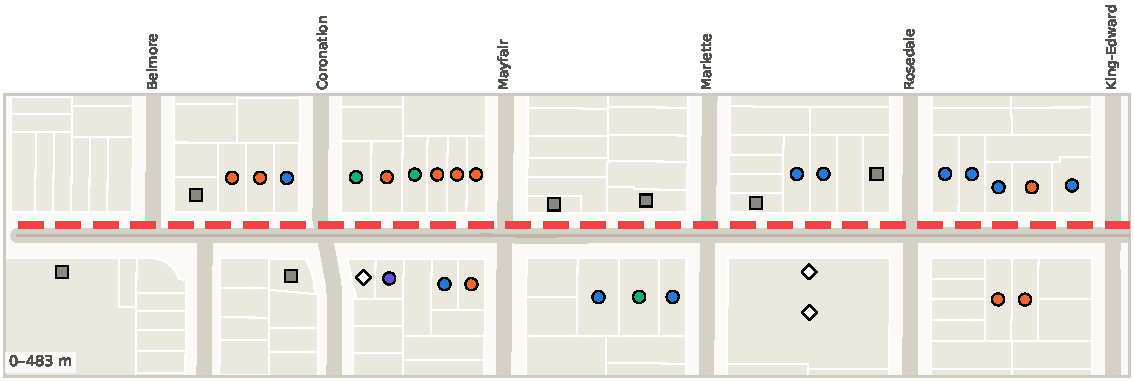
\includegraphics[width=\textwidth]{figures/panels/today_fr_p1.pdf}\\[1pt]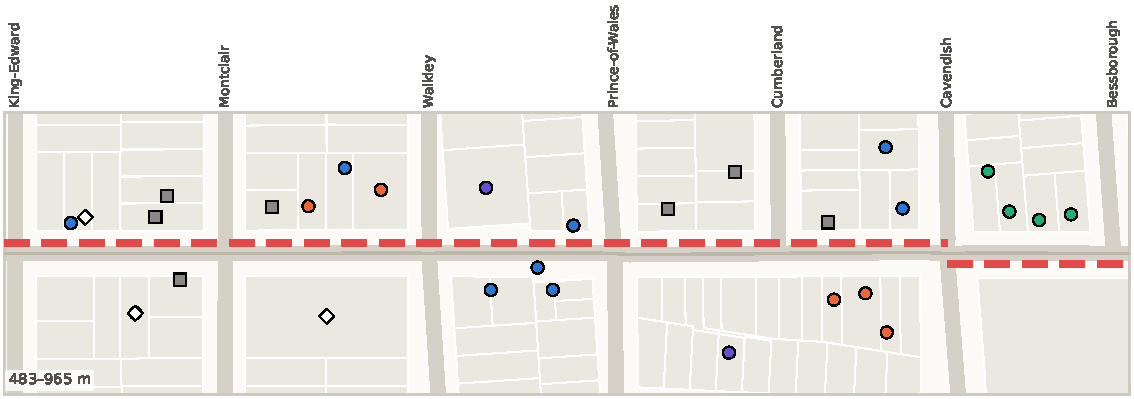
\includegraphics[width=\textwidth]{figures/panels/today_fr_p2.pdf}\\[1pt]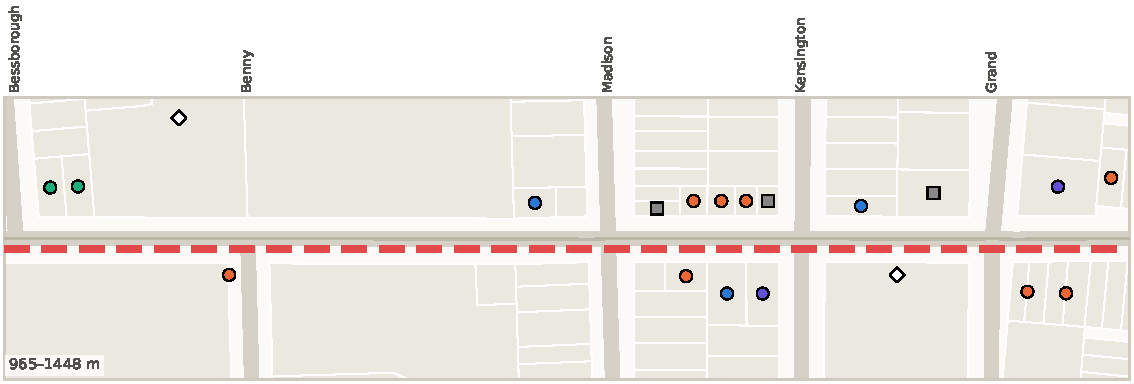
\includegraphics[width=\textwidth]{figures/panels/today_fr_p3.pdf}\end{center}
\vfill{\scriptsize Tirets rouges\,: le côté où la piste deviendrait du stationnement chaque hiver selon la proposition, telle que décrite par le conseiller. \textbf{(1/2)}}\\{\tiny Fond\,: données ouvertes de la Ville de Montréal, CC-BY 4.0 (géobase, rôle d'évaluation). Lecture\,: l'auteur. Imagerie\,: Gouvernement du Québec (Imagerie\_GQ, consultée le 25 oct. 2026). LiDAR\,: Ville de Montréal 2015, CC-BY 4.0.}\end{frame}
\begin{frame}{Sur le cadastre d'aujourd'hui\,: garage d'origine et entrée aujourd'hui}
\begin{center}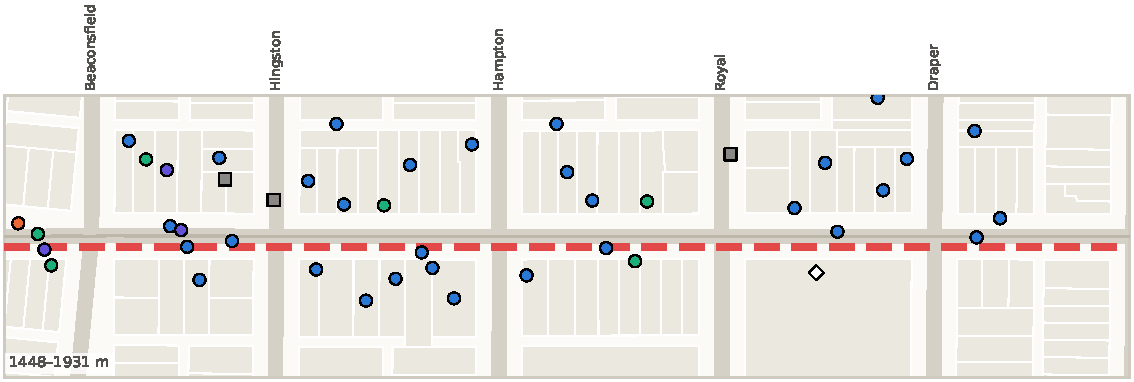
\includegraphics[width=\textwidth]{figures/panels/today_fr_p4.pdf}\\[1pt]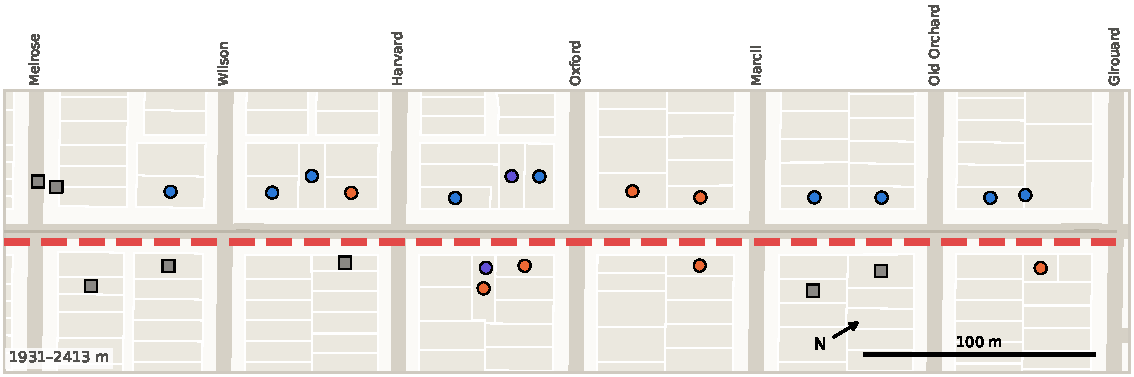
\includegraphics[width=\textwidth]{figures/panels/today_fr_p5.pdf}\\[3pt]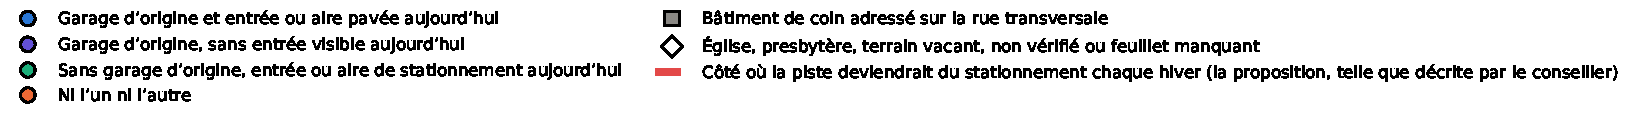
\includegraphics[width=0.95\textwidth]{figures/panels/today_fr_legend.pdf}\end{center}
\vfill{\scriptsize Tirets rouges\,: le côté où la piste deviendrait du stationnement chaque hiver selon la proposition, telle que décrite par le conseiller. \textbf{(2/2)}}\\{\tiny Fond\,: données ouvertes de la Ville de Montréal, CC-BY 4.0 (géobase, rôle d'évaluation). Lecture\,: l'auteur. Imagerie\,: Gouvernement du Québec (Imagerie\_GQ, consultée le 25 oct. 2026). LiDAR\,: Ville de Montréal 2015, CC-BY 4.0.}\end{frame}
\begin{frame}{Les plans de 1954--1955, géoréférencés\,: chaque garage porte le mot «\,Auto\,»}
\begin{center}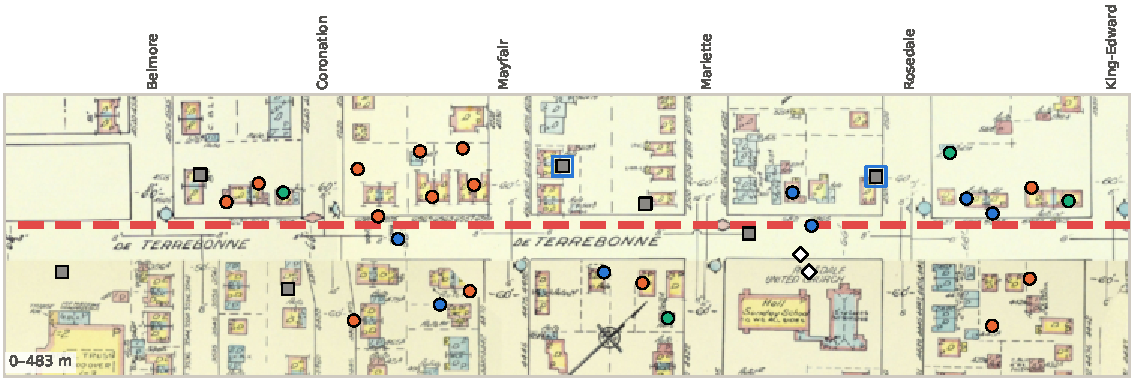
\includegraphics[width=\textwidth]{figures/panels/underwriters_fr_p1.pdf}\\[1pt]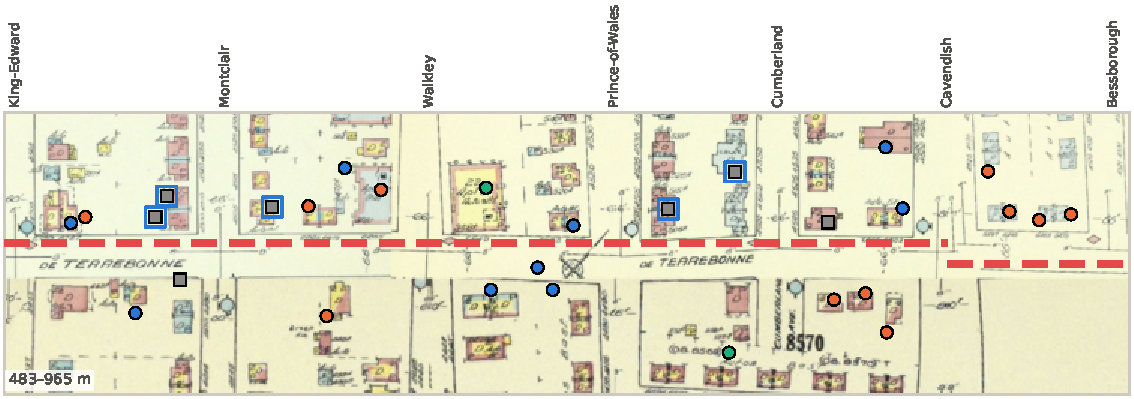
\includegraphics[width=\textwidth]{figures/panels/underwriters_fr_p2.pdf}\\[1pt]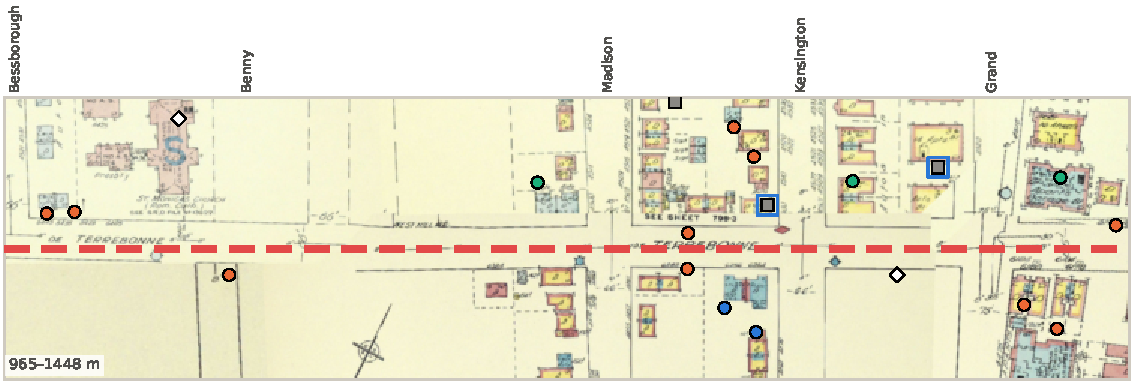
\includegraphics[width=\textwidth]{figures/panels/underwriters_fr_p3.pdf}\end{center}
\vfill{\scriptsize Les bandes de façade des feuillets, redressées le long de la rue; un repère par bâtiment (le blanc\,: le feuillet 787-8, manquant). \textbf{(1/2)}}\\{\tiny Source\,: Underwriters' Survey Bureau, Insurance plan of the city of Montreal, vol.~7, 1954--1955 (BAnQ, notice 0000174390). Lecture\,: l'auteur, une ligne par bâtiment.}\end{frame}
\begin{frame}{Les plans de 1954--1955, géoréférencés\,: chaque garage porte le mot «\,Auto\,»}
\begin{center}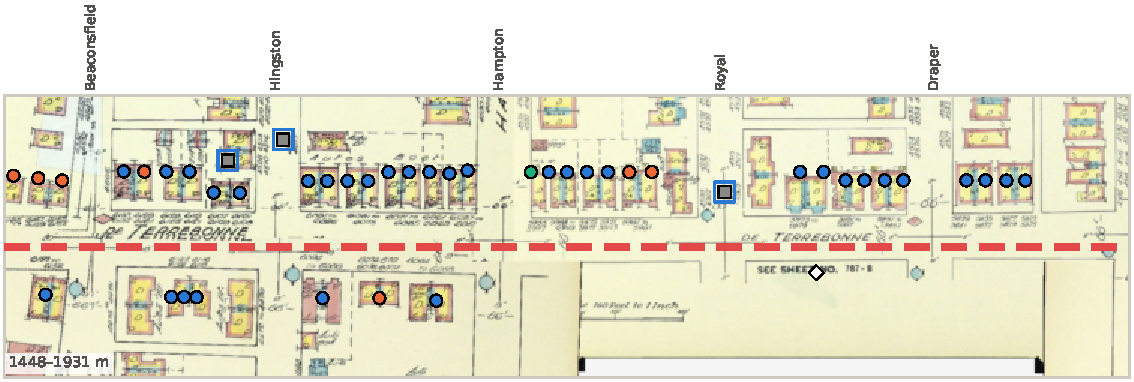
\includegraphics[width=\textwidth]{figures/panels/underwriters_fr_p4.pdf}\\[1pt]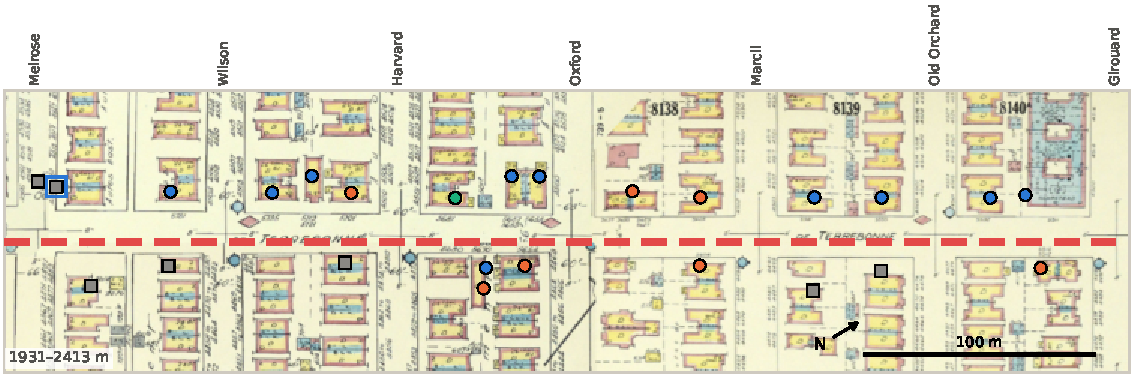
\includegraphics[width=\textwidth]{figures/panels/underwriters_fr_p5.pdf}\\[3pt]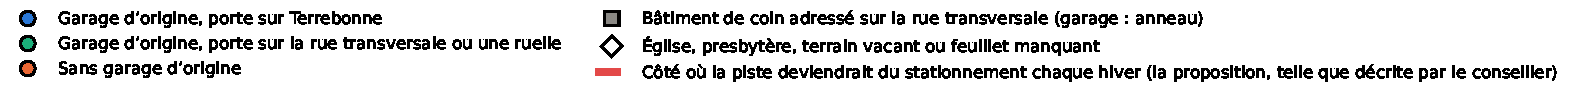
\includegraphics[width=0.95\textwidth]{figures/panels/underwriters_fr_legend.pdf}\end{center}
\vfill{\scriptsize Les bandes de façade des feuillets, redressées le long de la rue; un repère par bâtiment (le blanc\,: le feuillet 787-8, manquant). \textbf{(2/2)}}\\{\tiny Source\,: Underwriters' Survey Bureau, Insurance plan of the city of Montreal, vol.~7, 1954--1955 (BAnQ, notice 0000174390). Lecture\,: l'auteur, une ligne par bâtiment.}\end{frame}

\begin{frame}{Trois sources, un même repère}\begin{center}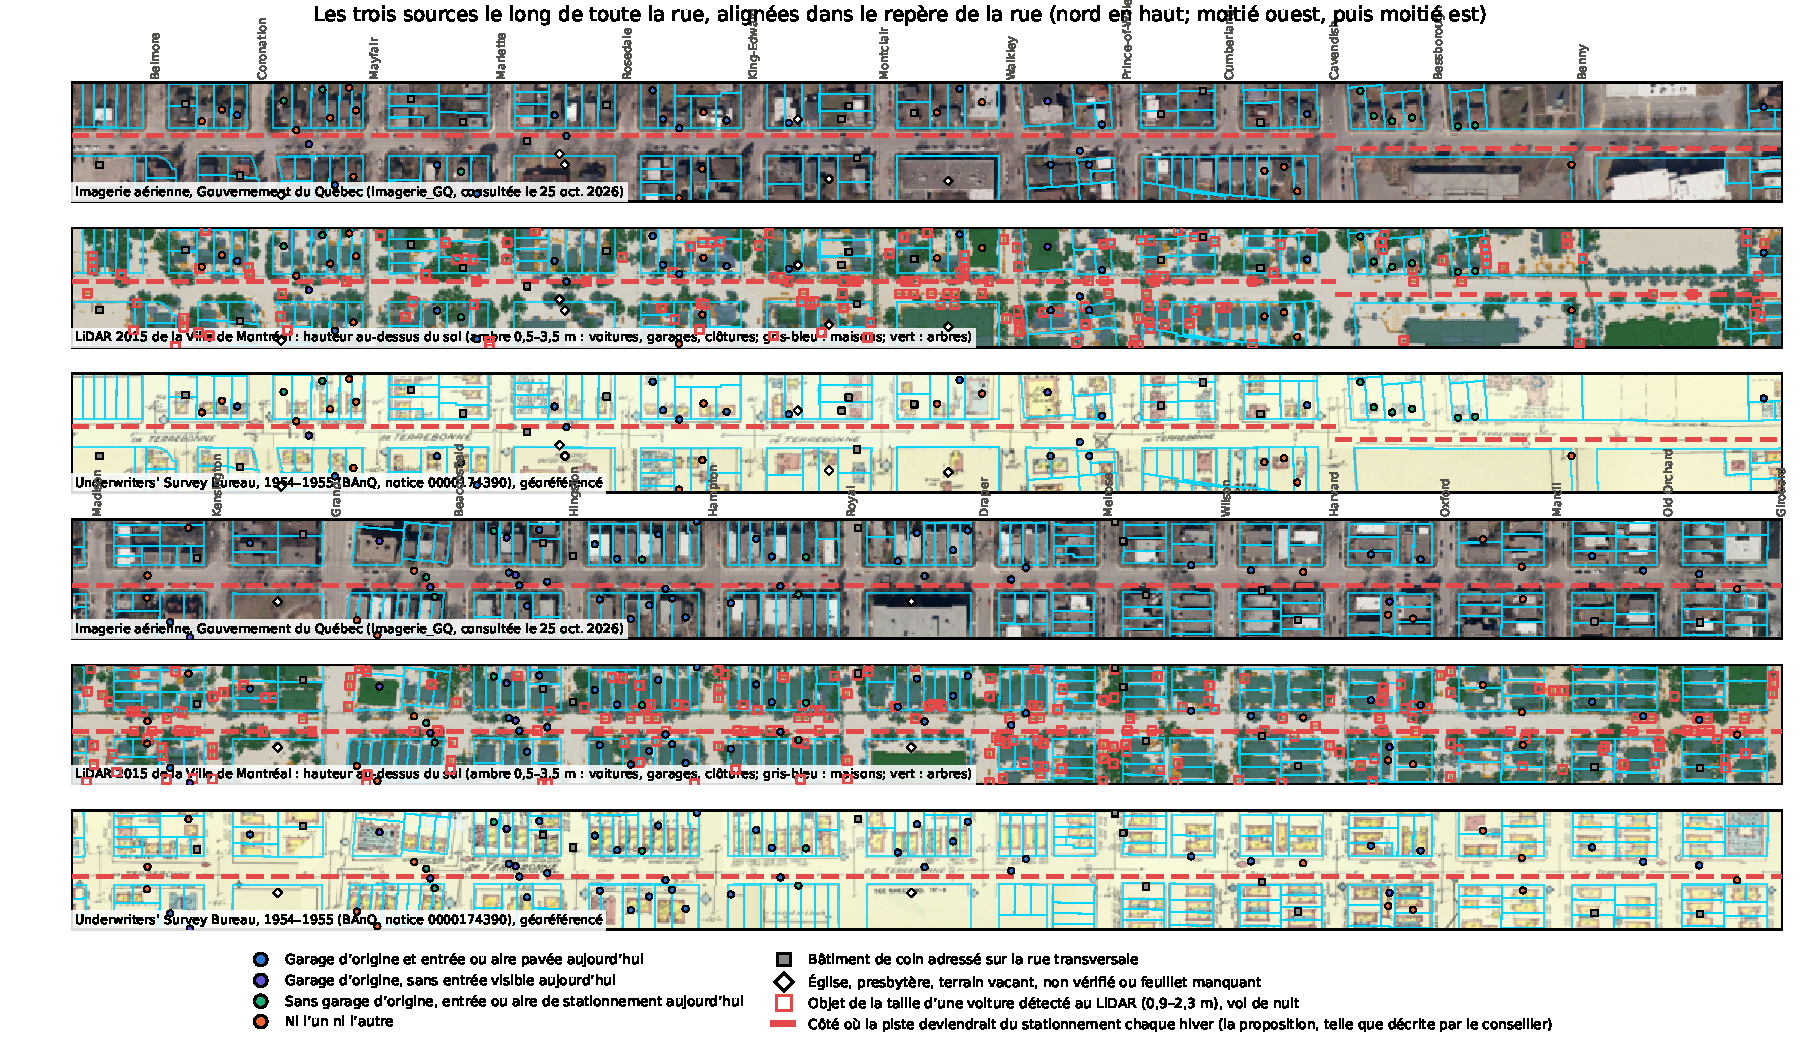
\includegraphics[height=0.74\textheight]{figures/method_overview_fr.pdf}\end{center}\vfill{\scriptsize Imagerie aérienne (optique), LiDAR 2015 de la Ville en hauteur au-dessus du sol, et feuillets de 1954--1955, tous géoréférencés dans le repère de la rue.}\\{\tiny Imagerie\,: Gouvernement du Québec (Imagerie\_GQ, consultée le 25 oct. 2026). LiDAR\,: Ville de Montréal 2015, CC-BY 4.0. Source\,: Underwriters' Survey Bureau, Insurance plan of the city of Montreal, vol.~7, 1954--1955 (BAnQ, notice 0000174390). Lecture\,: l'auteur, une ligne par bâtiment.}\end{frame}
\begin{frame}{Un îlot dans les trois sources\,: Hingston à Hampton}\begin{columns}[T]\column{0.42\textwidth}\centering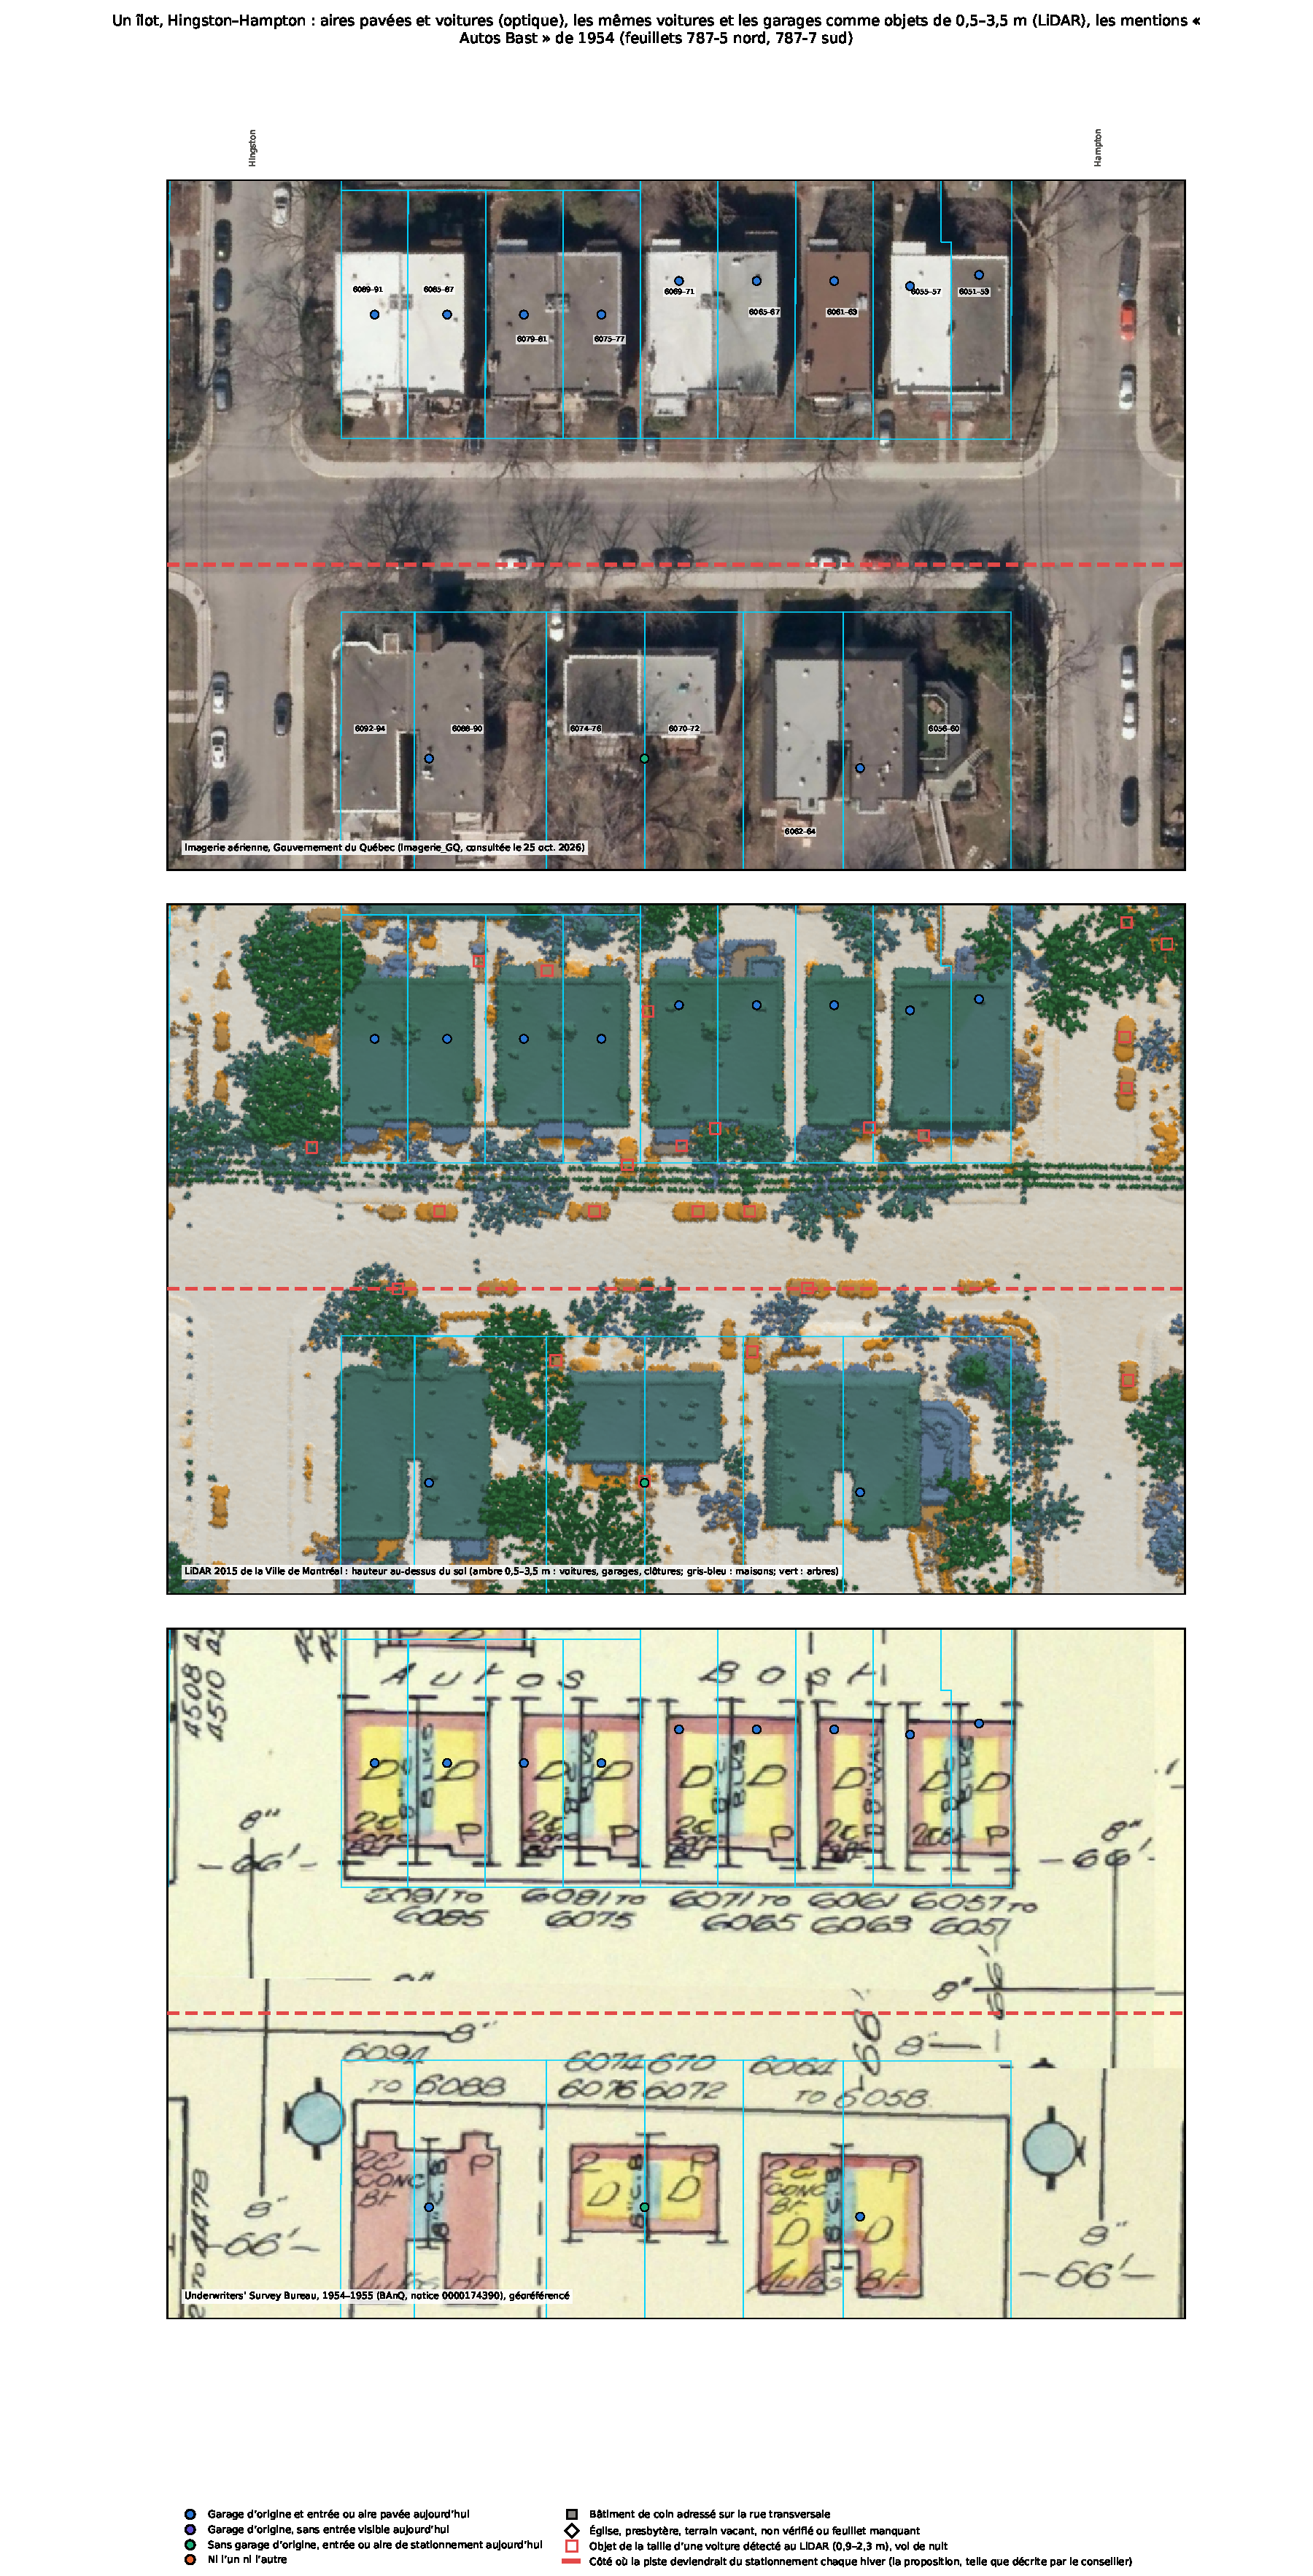
\includegraphics[height=0.74\textheight]{figures/method_detail_hingston_hampton_fr.pdf}\column{0.56\textwidth}{\small Aires pavées et voitures (optique); les mêmes voitures et les garages comme objets de 0,5--3,5\,m (LiDAR, carrés rouges = détections automatiques); les «\,Autos Bast\,» de 1954.}\end{columns}\vfill{\tiny Imagerie\,: Gouvernement du Québec (Imagerie\_GQ, consultée le 25 oct. 2026). LiDAR\,: Ville de Montréal 2015, CC-BY 4.0. Source\,: Underwriters' Survey Bureau, Insurance plan of the city of Montreal, vol.~7, 1954--1955 (BAnQ, notice 0000174390). Lecture\,: l'auteur, une ligne par bâtiment.}\end{frame}
\begin{frame}{Voitures stationnées dans la rue\,: deux acquisitions, deux moments}\begin{columns}[T]\column{0.45\textwidth}\begin{itemize}\item De jour, au printemps, après juin 2024 (imagerie)\,: 158 voitures sur Terrebonne (nord 30, sud 128)
\item Deux nuits de semaine, en 2015, avant la piste (LiDAR, dim.--lun. et lun.--mar., 0\,h--3\,h\,50)\,: 183 voitures sur Terrebonne à l'œil (nord 93, sud 90); un détecteur automatique en trouve 85, plus 253 objets de la taille d'une voiture sur les lots privés à moins de 45\,m et 70 sur les rues transversales
\item Dix ans et un réaménagement d'écart\,: chaque compte décrit son moment, pas un avant-après\end{itemize}\column{0.55\textwidth}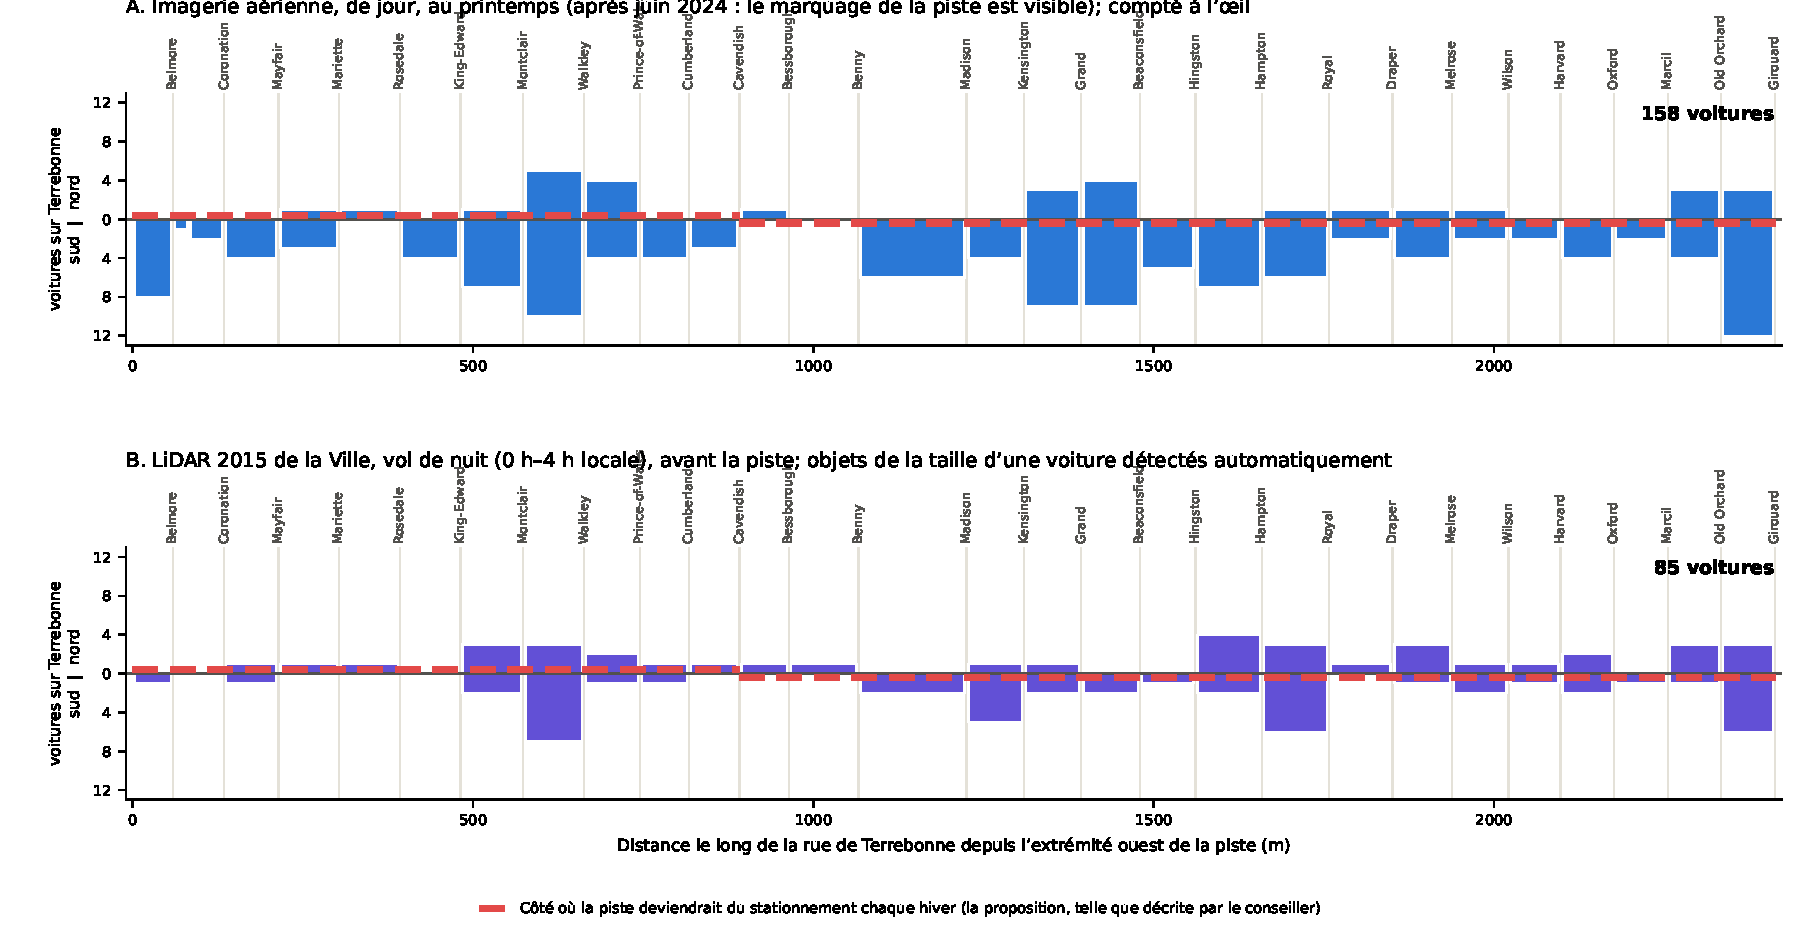
\includegraphics[width=\textwidth]{figures/terrebonne_on_street_cars_fr.pdf}\end{columns}\vfill{\tiny Imagerie\,: Gouvernement du Québec (Imagerie\_GQ, consultée le 25 oct. 2026). LiDAR\,: Ville de Montréal 2015, CC-BY 4.0.}\end{frame}
\begin{frame}{Où étaient les voitures\,: les deux acquisitions, panneau par panneau}\begin{center}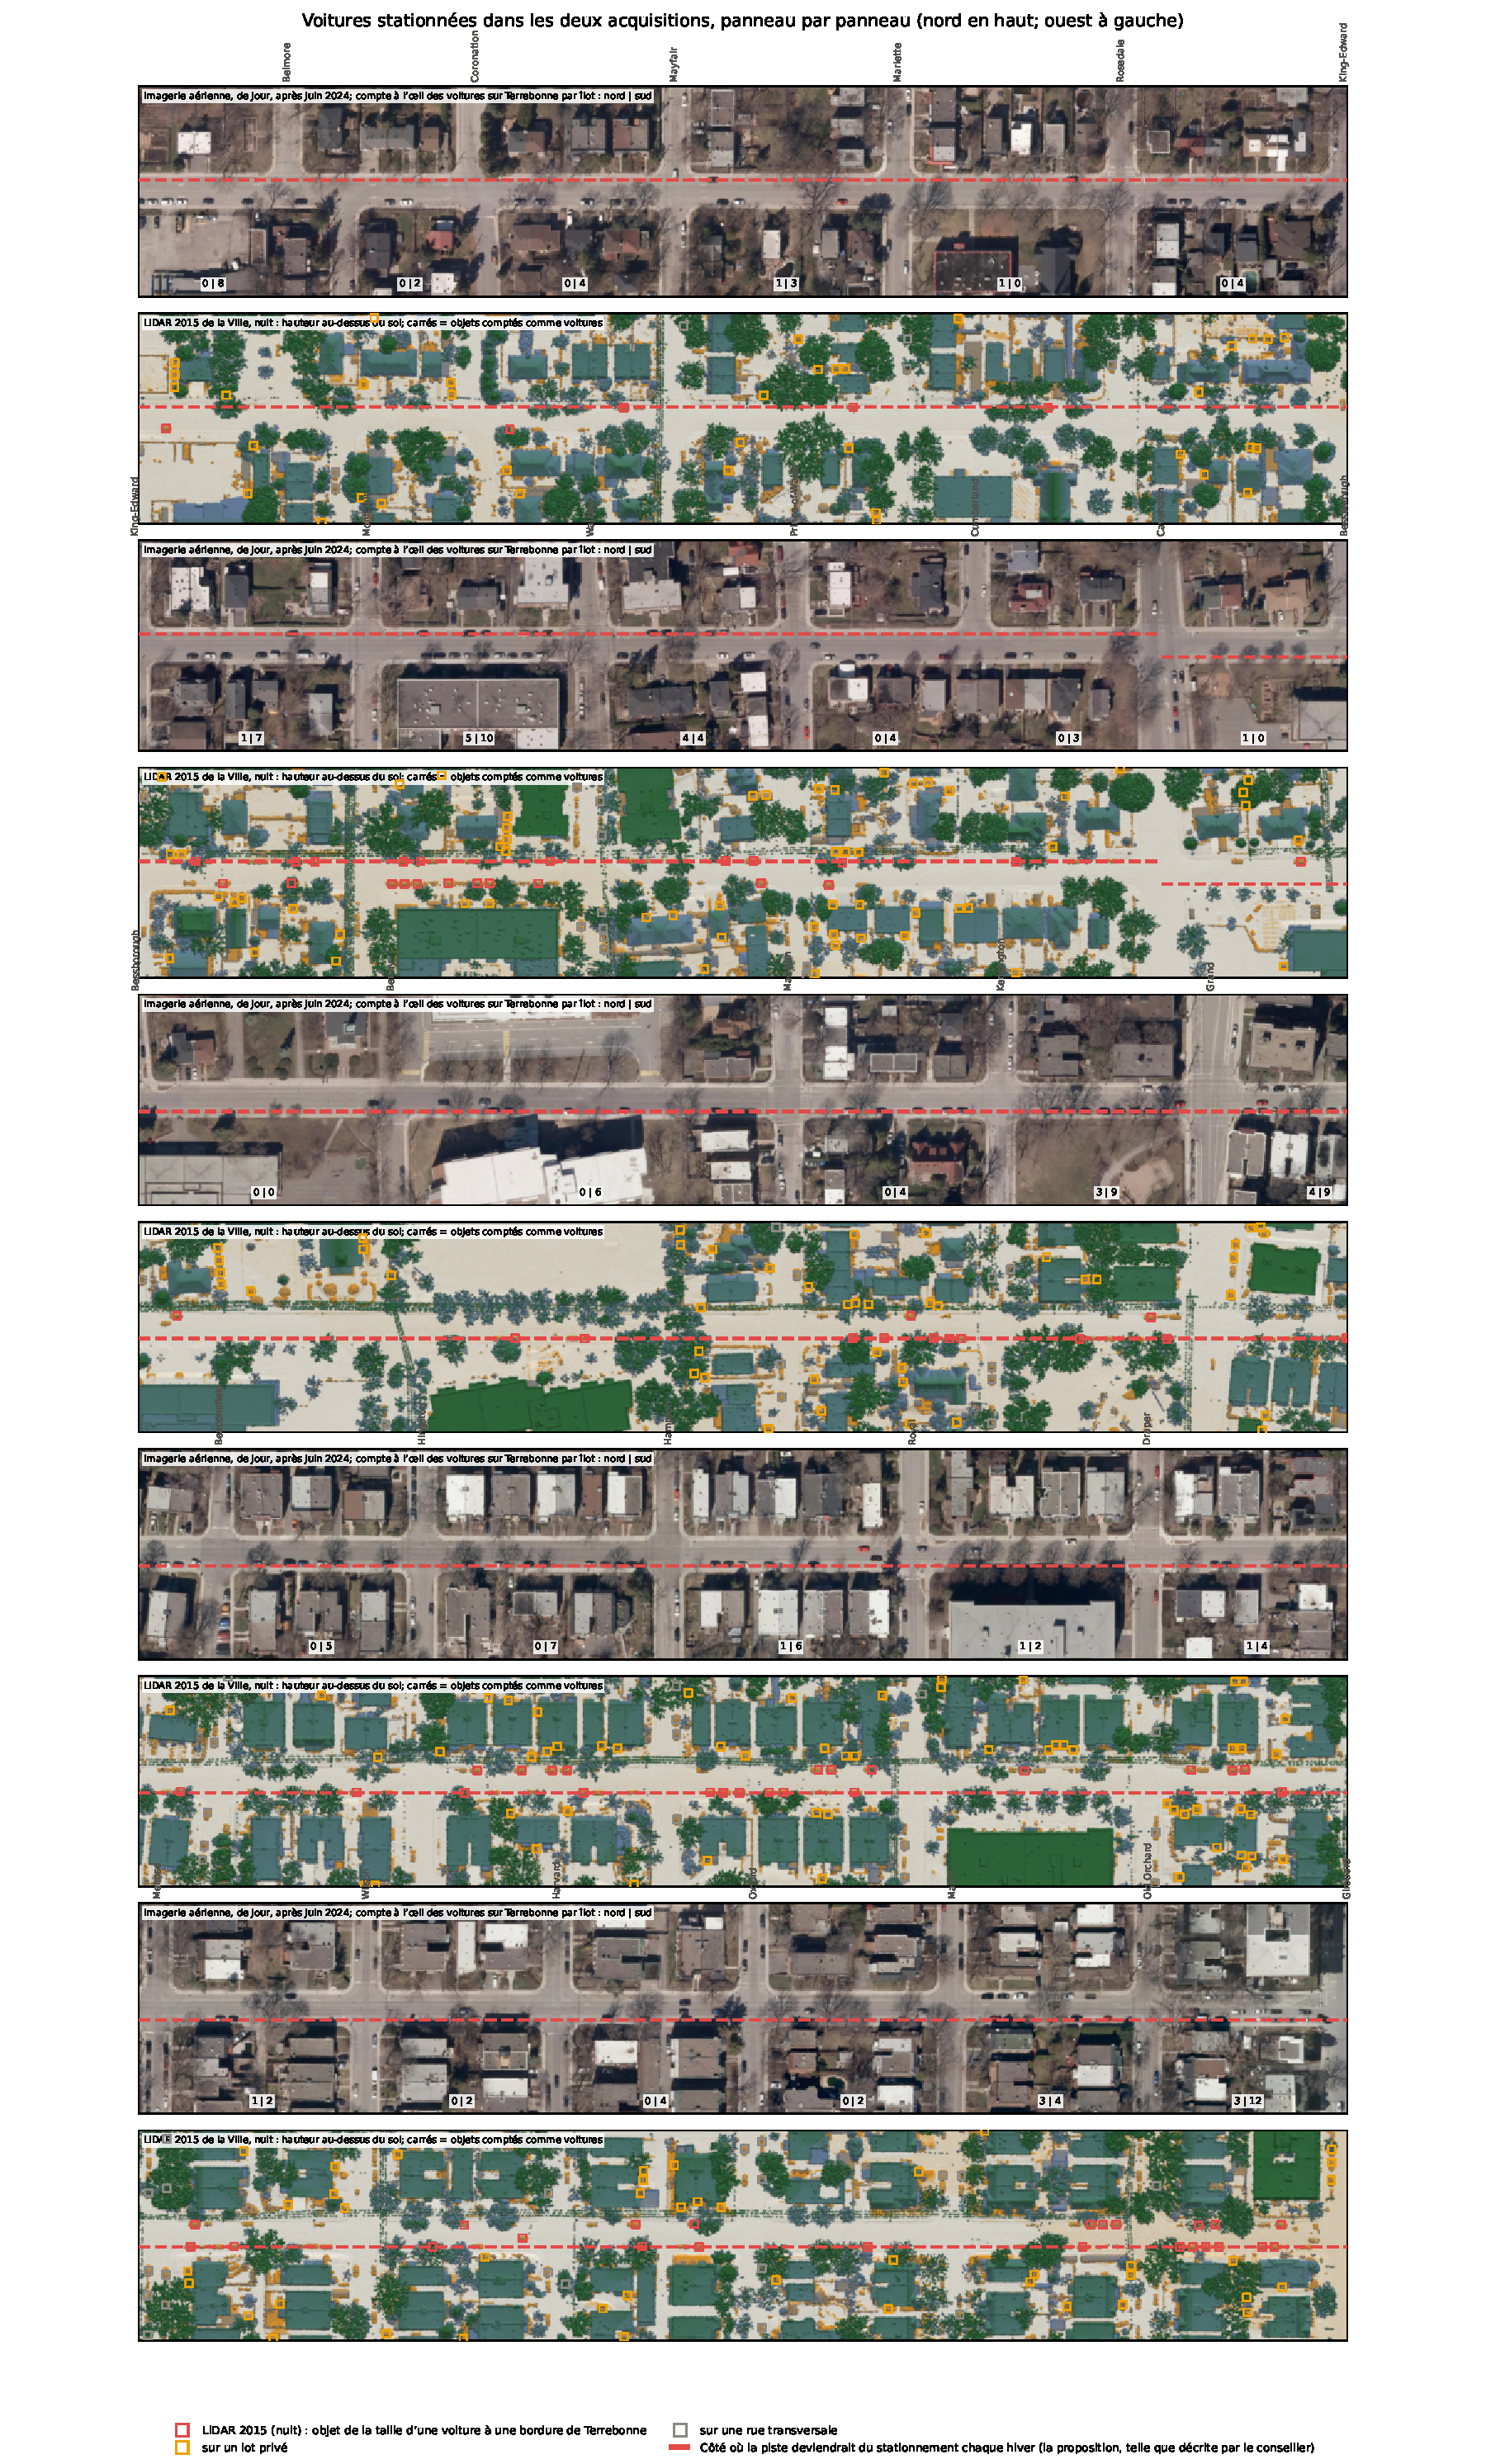
\includegraphics[height=0.74\textheight]{figures/terrebonne_parked_cars_strips_fr.pdf}\end{center}\vfill{\scriptsize Image de jour (compte à l'œil par îlot, nord | sud) au-dessus du raster de hauteur de nuit 2015; carrés = voitures du détecteur (rouge à une bordure de Terrebonne, orange sur un lot, gris sur une rue transversale).}\\{\tiny Imagerie\,: Gouvernement du Québec (Imagerie\_GQ, consultée le 25 oct. 2026). LiDAR\,: Ville de Montréal 2015, CC-BY 4.0.}\end{frame}
\begin{frame}{Chaque objet de la taille d'une voiture trouvé par le détecteur dans le LiDAR de nuit, sur le cadastre d'aujourd'hui}\begin{center}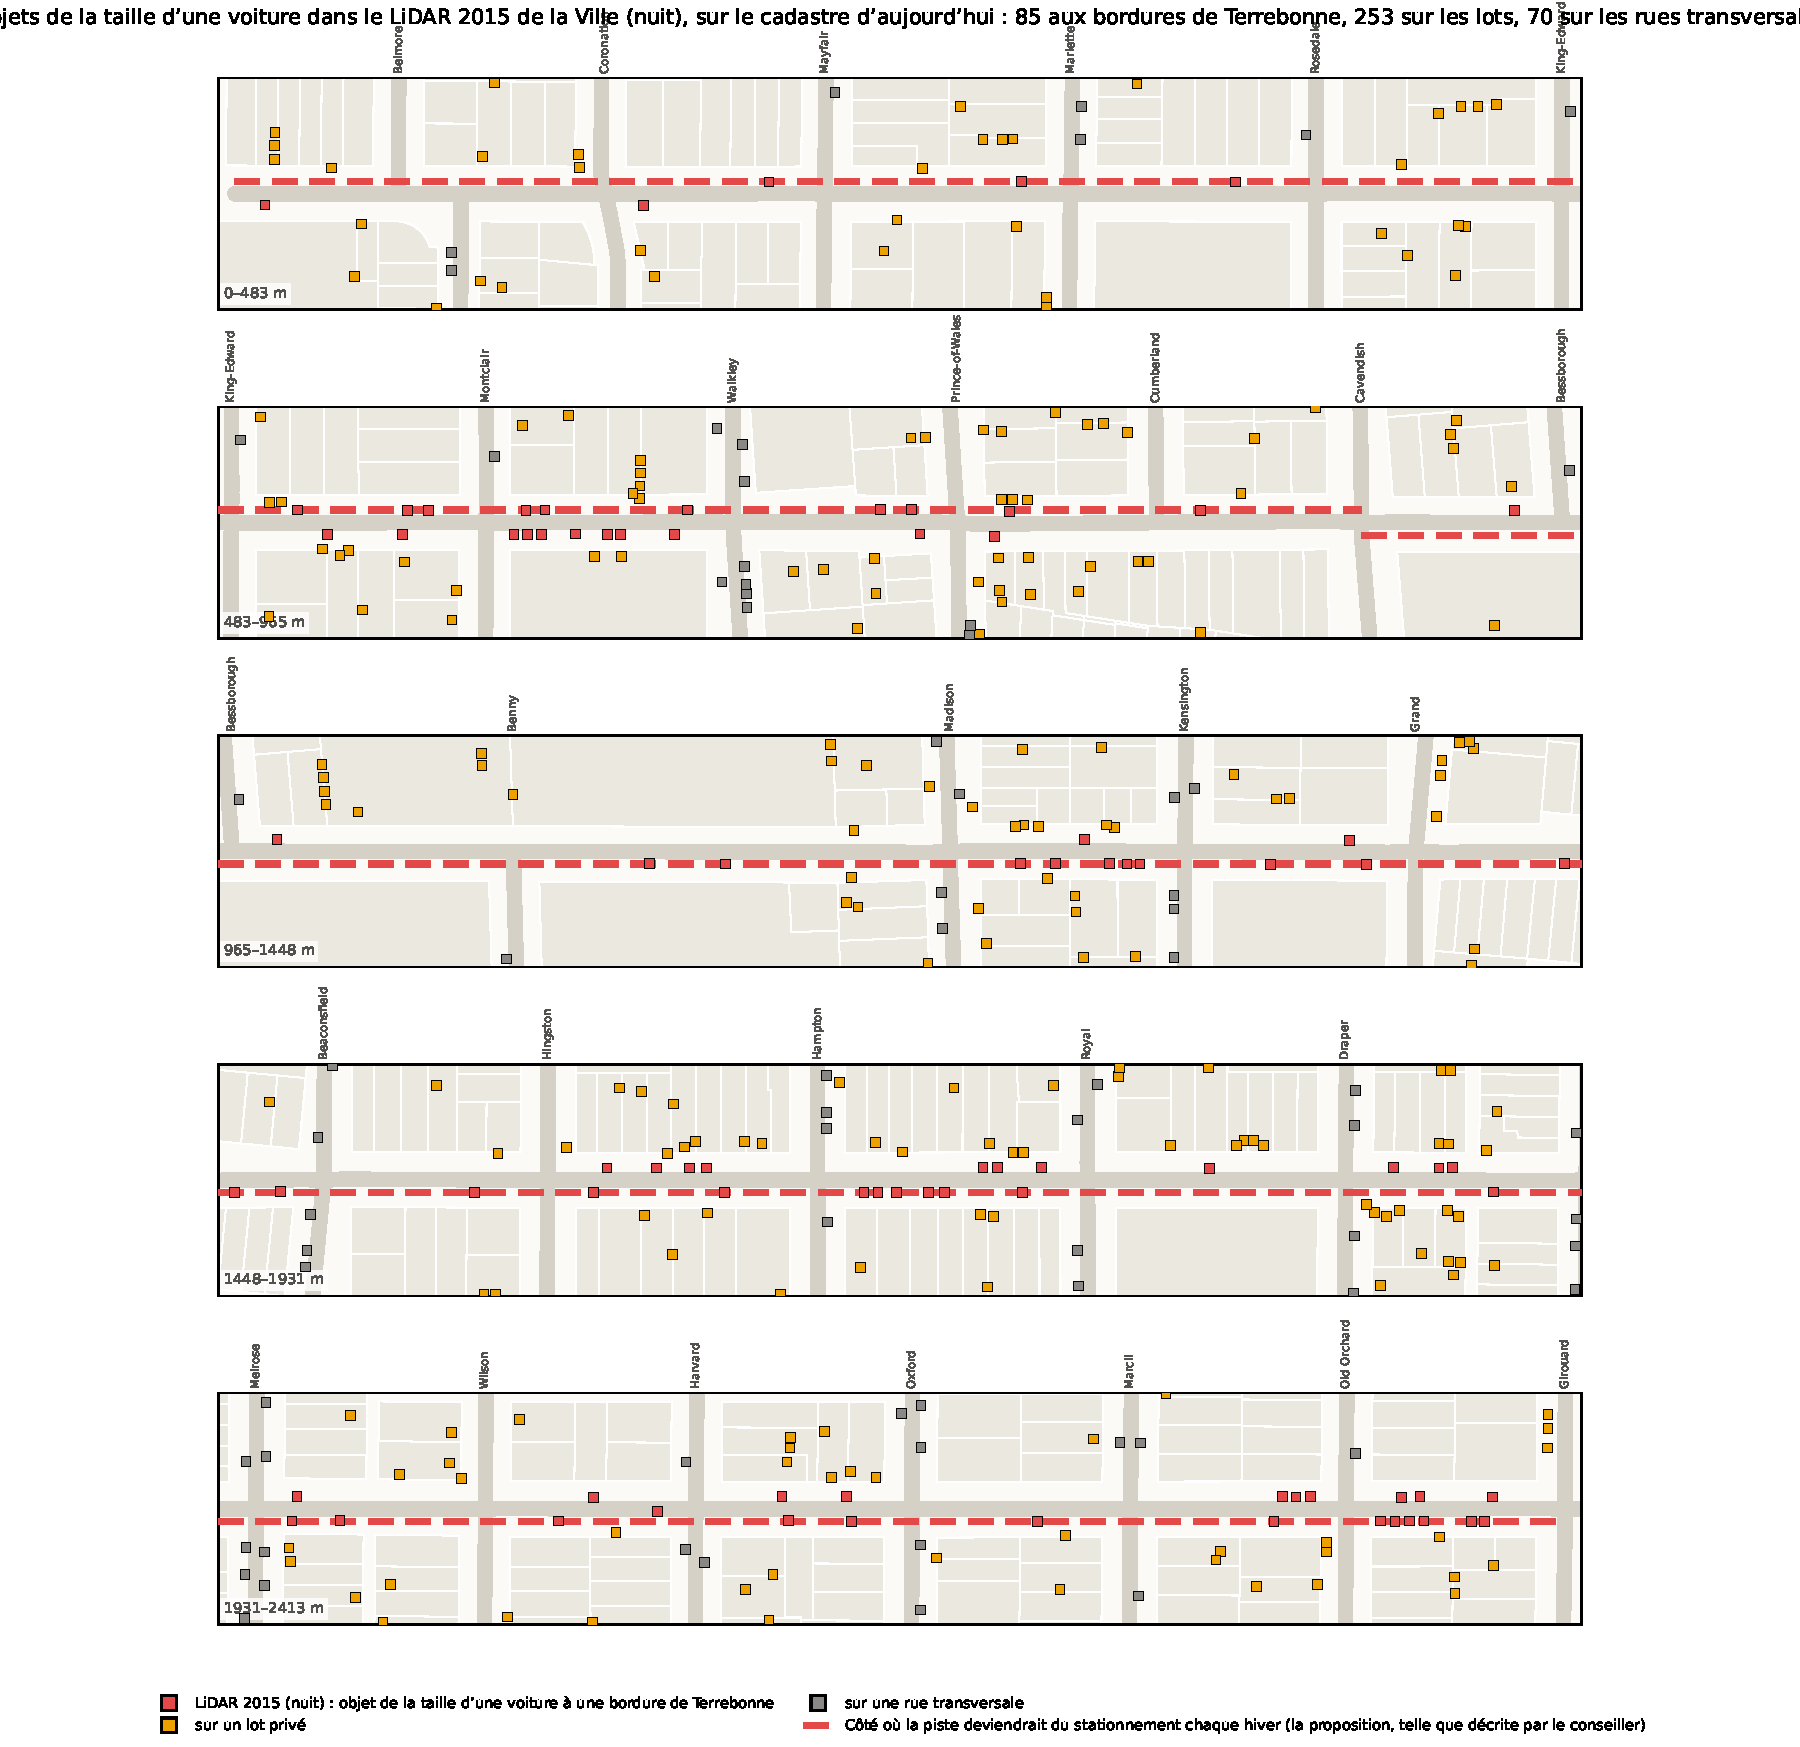
\includegraphics[height=0.78\textheight]{figures/terrebonne_parked_cars_lidar_map_fr.pdf}\end{center}\vfill{\tiny Imagerie\,: Gouvernement du Québec (Imagerie\_GQ, consultée le 25 oct. 2026). LiDAR\,: Ville de Montréal 2015, CC-BY 4.0.}\end{frame}
\begin{frame}{À quoi ressemble une détection de voiture au LiDAR}\begin{center}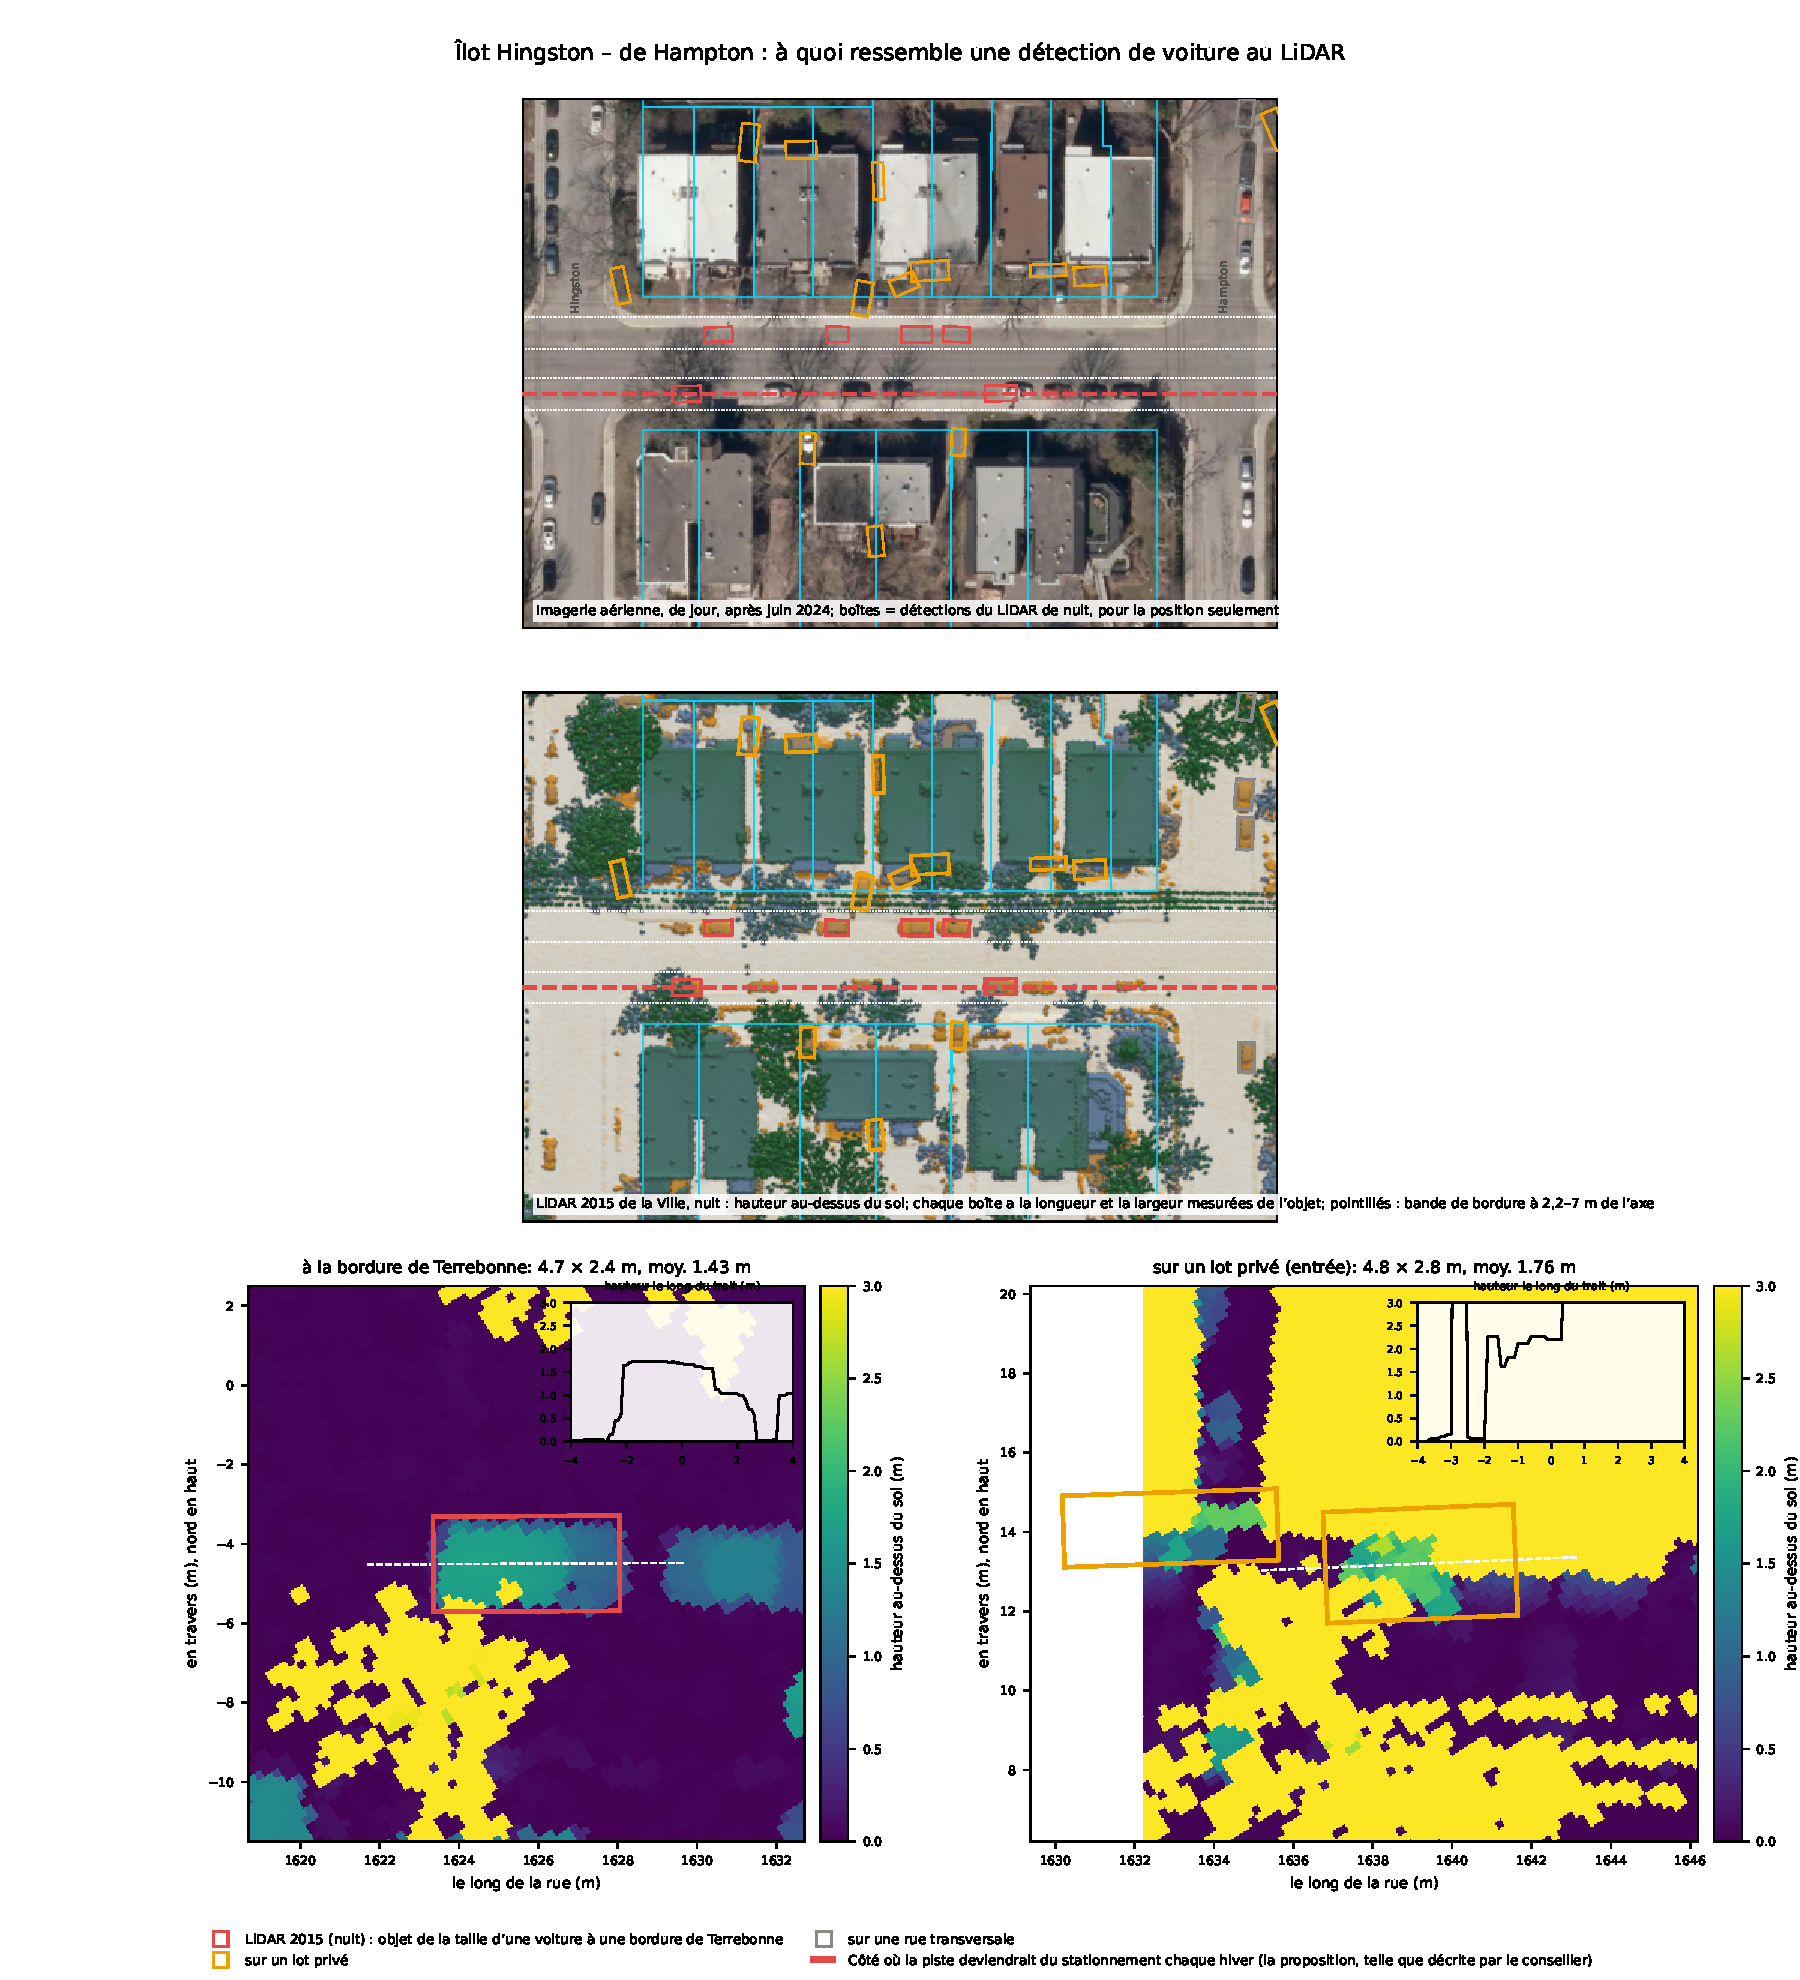
\includegraphics[height=0.74\textheight]{figures/terrebonne_parked_cars_closeup_hingston_fr.pdf}\end{center}\vfill{\scriptsize Chaque boîte a la longueur et la largeur mesurées de l'objet; les pointillés bornent la bande de bordure (2,2--7\,m de l'axe) qui sépare la rue du lot. En bas\,: une voiture à la bordure et une dans une entrée à 40 px/m, avec la hauteur en mètres; un toit plat à 1,4--1,5\,m sur environ 4,5\,m.}\\{\tiny Imagerie\,: Gouvernement du Québec (Imagerie\_GQ, consultée le 25 oct. 2026). LiDAR\,: Ville de Montréal 2015, CC-BY 4.0.}\end{frame}
\begin{frame}{Vérifications de la méthode}\begin{itemize}\item Géoréférencement\,: chaque feuillet ajusté sur ses intersections, résidus sous 3,3\,m sur 14 des 16 feuillets (7\,m en un point); vérifié contre le cadastre de la Ville sur chaque feuillet
\item La lecture de 1954--1955 concorde avec les marques indépendantes de l'auteur de juin 2024 sur les 126 bâtiments
\item La lecture actuelle\,: un lecteur, gradée ligne par ligne, relisible à partir de l'imagerie publique; faite avant que le côté converti soit tracé
\item Détecteur de voitures LiDAR vérifié à l'œil sur les 29 îlots\,: 85 objets trouvés sur 183 aux bordures (46\,\%); c'est le compte à l'œil qui est rapporté
\item Un recensement de la façade, pas un échantillon; chaque nombre produit par un script à partir de données publiques\end{itemize}\end{frame}
\begin{frame}{Réserves}\begin{itemize}\item Garages d'origine, pas entrées\,: la part de 1954--1955 est une borne inférieure
\item D'origine, visible\,: aucune lecture ne voit l'intérieur d'un garage (atelier, rangement, pièce habitable); un garage de 1930 peut être trop petit pour les véhicules d'aujourd'hui
\item Bâtiments, pas ménages\,: un duplex jumelé compte deux à quatre logements et un ou deux garages
\item Un feuillet manquant en 1954--1955 (côté sud, Hampton à Melrose); les lectures de confiance moyenne ou incertaines sont signalées ligne par ligne
\item Tout est dans le tableau\,: une ligne par bâtiment, vérifiable par adresse\end{itemize}\end{frame}
\begin{frame}{Où trouver le tout}\begin{itemize}\item Page web, note, cartes, tableaux\,: \url{https://openmobilitydata.github.io/Terrebonne-open-sources/1954-underwriters-plans-terrebonne-garages/}
\item Les feuillets eux-mêmes\,: BAnQ numérique, \url{https://collections.banq.qc.ca/ark:/52327/2244199}
\item Dépôt\,: \url{https://github.com/OpenMobilityData/Terrebonne-open-sources}\end{itemize}\vfill{\tiny Source\,: Underwriters' Survey Bureau, Insurance plan of the city of Montreal, vol.~7, 1954--1955 (BAnQ, notice 0000174390). Lecture\,: l'auteur, une ligne par bâtiment. Fond\,: données ouvertes de la Ville de Montréal, CC-BY 4.0 (géobase, rôle d'évaluation). Lecture\,: l'auteur. Imagerie\,: Gouvernement du Québec (Imagerie\_GQ, consultée le 25 oct. 2026). LiDAR\,: Ville de Montréal 2015, CC-BY 4.0.}\end{frame}
\end{document}
